% Options for packages loaded elsewhere
\PassOptionsToPackage{unicode}{hyperref}
\PassOptionsToPackage{hyphens}{url}
%
\documentclass[
  8pt,
  ignorenonframetext,
]{beamer}
\usepackage{pgfpages}
\setbeamertemplate{caption}[numbered]
\setbeamertemplate{caption label separator}{: }
\setbeamercolor{caption name}{fg=normal text.fg}
\beamertemplatenavigationsymbolsempty
% Prevent slide breaks in the middle of a paragraph
\widowpenalties 1 10000
\raggedbottom
\setbeamertemplate{part page}{
  \centering
  \begin{beamercolorbox}[sep=16pt,center]{part title}
    \usebeamerfont{part title}\insertpart\par
  \end{beamercolorbox}
}
\setbeamertemplate{section page}{
  \centering
  \begin{beamercolorbox}[sep=12pt,center]{part title}
    \usebeamerfont{section title}\insertsection\par
  \end{beamercolorbox}
}
\setbeamertemplate{subsection page}{
  \centering
  \begin{beamercolorbox}[sep=8pt,center]{part title}
    \usebeamerfont{subsection title}\insertsubsection\par
  \end{beamercolorbox}
}
\AtBeginPart{
  \frame{\partpage}
}
\AtBeginSection{
  \ifbibliography
  \else
    \frame{\sectionpage}
  \fi
}
\AtBeginSubsection{
  \frame{\subsectionpage}
}
\usepackage{amsmath,amssymb}
\usepackage{lmodern}
\usepackage{iftex}
\ifPDFTeX
  \usepackage[T1]{fontenc}
  \usepackage[utf8]{inputenc}
  \usepackage{textcomp} % provide euro and other symbols
\else % if luatex or xetex
  \usepackage{unicode-math}
  \defaultfontfeatures{Scale=MatchLowercase}
  \defaultfontfeatures[\rmfamily]{Ligatures=TeX,Scale=1}
\fi
% Use upquote if available, for straight quotes in verbatim environments
\IfFileExists{upquote.sty}{\usepackage{upquote}}{}
\IfFileExists{microtype.sty}{% use microtype if available
  \usepackage[]{microtype}
  \UseMicrotypeSet[protrusion]{basicmath} % disable protrusion for tt fonts
}{}
\makeatletter
\@ifundefined{KOMAClassName}{% if non-KOMA class
  \IfFileExists{parskip.sty}{%
    \usepackage{parskip}
  }{% else
    \setlength{\parindent}{0pt}
    \setlength{\parskip}{6pt plus 2pt minus 1pt}}
}{% if KOMA class
  \KOMAoptions{parskip=half}}
\makeatother
\usepackage{xcolor}
\newif\ifbibliography
\usepackage{color}
\usepackage{fancyvrb}
\newcommand{\VerbBar}{|}
\newcommand{\VERB}{\Verb[commandchars=\\\{\}]}
\DefineVerbatimEnvironment{Highlighting}{Verbatim}{commandchars=\\\{\}}
% Add ',fontsize=\small' for more characters per line
\usepackage{framed}
\definecolor{shadecolor}{RGB}{248,248,248}
\newenvironment{Shaded}{\begin{snugshade}}{\end{snugshade}}
\newcommand{\AlertTok}[1]{\textcolor[rgb]{0.94,0.16,0.16}{#1}}
\newcommand{\AnnotationTok}[1]{\textcolor[rgb]{0.56,0.35,0.01}{\textbf{\textit{#1}}}}
\newcommand{\AttributeTok}[1]{\textcolor[rgb]{0.77,0.63,0.00}{#1}}
\newcommand{\BaseNTok}[1]{\textcolor[rgb]{0.00,0.00,0.81}{#1}}
\newcommand{\BuiltInTok}[1]{#1}
\newcommand{\CharTok}[1]{\textcolor[rgb]{0.31,0.60,0.02}{#1}}
\newcommand{\CommentTok}[1]{\textcolor[rgb]{0.56,0.35,0.01}{\textit{#1}}}
\newcommand{\CommentVarTok}[1]{\textcolor[rgb]{0.56,0.35,0.01}{\textbf{\textit{#1}}}}
\newcommand{\ConstantTok}[1]{\textcolor[rgb]{0.00,0.00,0.00}{#1}}
\newcommand{\ControlFlowTok}[1]{\textcolor[rgb]{0.13,0.29,0.53}{\textbf{#1}}}
\newcommand{\DataTypeTok}[1]{\textcolor[rgb]{0.13,0.29,0.53}{#1}}
\newcommand{\DecValTok}[1]{\textcolor[rgb]{0.00,0.00,0.81}{#1}}
\newcommand{\DocumentationTok}[1]{\textcolor[rgb]{0.56,0.35,0.01}{\textbf{\textit{#1}}}}
\newcommand{\ErrorTok}[1]{\textcolor[rgb]{0.64,0.00,0.00}{\textbf{#1}}}
\newcommand{\ExtensionTok}[1]{#1}
\newcommand{\FloatTok}[1]{\textcolor[rgb]{0.00,0.00,0.81}{#1}}
\newcommand{\FunctionTok}[1]{\textcolor[rgb]{0.00,0.00,0.00}{#1}}
\newcommand{\ImportTok}[1]{#1}
\newcommand{\InformationTok}[1]{\textcolor[rgb]{0.56,0.35,0.01}{\textbf{\textit{#1}}}}
\newcommand{\KeywordTok}[1]{\textcolor[rgb]{0.13,0.29,0.53}{\textbf{#1}}}
\newcommand{\NormalTok}[1]{#1}
\newcommand{\OperatorTok}[1]{\textcolor[rgb]{0.81,0.36,0.00}{\textbf{#1}}}
\newcommand{\OtherTok}[1]{\textcolor[rgb]{0.56,0.35,0.01}{#1}}
\newcommand{\PreprocessorTok}[1]{\textcolor[rgb]{0.56,0.35,0.01}{\textit{#1}}}
\newcommand{\RegionMarkerTok}[1]{#1}
\newcommand{\SpecialCharTok}[1]{\textcolor[rgb]{0.00,0.00,0.00}{#1}}
\newcommand{\SpecialStringTok}[1]{\textcolor[rgb]{0.31,0.60,0.02}{#1}}
\newcommand{\StringTok}[1]{\textcolor[rgb]{0.31,0.60,0.02}{#1}}
\newcommand{\VariableTok}[1]{\textcolor[rgb]{0.00,0.00,0.00}{#1}}
\newcommand{\VerbatimStringTok}[1]{\textcolor[rgb]{0.31,0.60,0.02}{#1}}
\newcommand{\WarningTok}[1]{\textcolor[rgb]{0.56,0.35,0.01}{\textbf{\textit{#1}}}}
\setlength{\emergencystretch}{3em} % prevent overfull lines
\providecommand{\tightlist}{%
  \setlength{\itemsep}{0pt}\setlength{\parskip}{0pt}}
\setcounter{secnumdepth}{-\maxdimen} % remove section numbering
% type setting
% ------------------------------------------------------------------------------
\usepackage[german]{babel}     

% fonts
% ------------------------------------------------------------------------------
\usefonttheme{professionalfonts}

% slide title and horizontal line
% ------------------------------------------------------------------------------
\setbeamertemplate{frametitle}{%
    \vskip-30pt \color{black}\large%
    \begin{minipage}[b][23pt]{120mm}%
    \flushleft\insertframetitle%
    \end{minipage}%
}

\setbeamertemplate{headline}										
{
\vskip10pt\hfill\hspace{3.5mm} 										 
\vskip15pt\color{black}\rule{\textwidth}{0.4pt} 					 
}

% slide number
% ---------------------------------------------------------------
\setbeamertemplate{navigation symbols}{}
\setbeamertemplate{footline}
{
\vskip5pt
\vskip2pt
\makebox[123mm]{\hspace{7.5mm}
\hfill Multivariate Datenanalyse $\vert$ 
\copyright $ $ 2023 Dirk Ostwald CC BY-NC-SA 4.0 $\vert$ 
Folie \insertframenumber}
\vskip4pt
}

% block color scheme
% ------------------------------------------------------------------------------
% colors
\definecolor{white}{RGB}{255,255,255}
\definecolor{grey}{RGB}{235,235,235}
\definecolor{lightgrey}{RGB}{245,245,245}
\definecolor{LightBlue}{RGB}{220,220,255}
\definecolor{darkblue}{RGB}{51, 51, 153}

% definitions and theorems
\setbeamercolor{block title}{fg = black, bg = grey}
\setbeamercolor{block body}{fg = black, bg = lightgrey}

% general line spacing 
% ------------------------------------------------------------------------------
\linespread{1.3}

% local line spacing
% ------------------------------------------------------------------------------
\usepackage{setspace}

% colors
% -----------------------------------------------------------------------------
\usepackage{color}

% justified text
% ------------------------------------------------------------------------------
\usepackage{ragged2e}
\usepackage{etoolbox}
\apptocmd{\frame}{}{\justifying}{}

% bullet point lists
% -----------------------------------------------------------------------------
\setbeamertemplate{itemize item}[circle]
\setbeamertemplate{itemize subitem}[circle]
\setbeamertemplate{itemize subsubitem}[circle]
\setbeamercolor{itemize item}{fg = black}
\setbeamercolor{itemize subitem}{fg = black}
\setbeamercolor{itemize subsubitem}{fg = black}
\setbeamercolor{enumerate item}{fg = black}
\setbeamercolor{enumerate subitem}{fg = black}
\setbeamercolor{enumerate subsubitem}{fg = black}
\setbeamerfont{itemize/enumerate body}{}
\setbeamerfont{itemize/enumerate subbody}{size = \normalsize}
\setbeamerfont{itemize/enumerate subsubbody}{size = \normalsize}

% color links
% ------------------------------------------------------------------------------
\usepackage{hyperref}
\definecolor{urls}{RGB}{204,0,0}
\hypersetup{colorlinks, citecolor = darkblue, urlcolor = urls}


% additional math commands
% ------------------------------------------------------------------------------
\usepackage{bm}                                         % bold math symbols
\newcommand{\niton}{\not\owns}

% text highlighting
% ------------------------------------------------------------------------------
\usepackage{soul}
\makeatletter
\let\HL\hl
\renewcommand\hl{%
  \let\set@color\beamerorig@set@color
  \let\reset@color\beamerorig@reset@color
  \HL}
\makeatother

% equation highlighting
% -----------------------------------------------------------------------------
\newcommand{\highlight}[2][yellow]{\mathchoice%
  {\colorbox{#1}{$\displaystyle#2$}}%
  {\colorbox{#1}{$\textstyle#2$}}%
  {\colorbox{#1}{$\scriptstyle#2$}}%
  {\colorbox{#1}{$\scriptscriptstyle#2$}}}%

% additional mathematical operators
% ------------------------------------------------------------------------------
\DeclareMathOperator*{\argmax}{arg\,max}
\DeclareMathOperator*{\argmin}{arg\,min}

\ifLuaTeX
  \usepackage{selnolig}  % disable illegal ligatures
\fi
\IfFileExists{bookmark.sty}{\usepackage{bookmark}}{\usepackage{hyperref}}
\IfFileExists{xurl.sty}{\usepackage{xurl}}{} % add URL line breaks if available
\urlstyle{same} % disable monospaced font for URLs
\hypersetup{
  hidelinks,
  pdfcreator={LaTeX via pandoc}}

\author{}
\date{\vspace{-2.5em}}

\begin{document}

\begin{frame}[plain]{}
\protect\hypertarget{section}{}
\center

\begin{center}
\includegraphics[width=0.2\linewidth]{2_Abbildungen/mvda_2_otto} \end{center}

\vspace{2mm}

\Huge

Multivariate Datenanalyse \vspace{6mm}

\Large

MSc Psychologie WiSe 2022/23

\vspace{6mm}
\large

Prof.~Dr.~Dirk Ostwald
\end{frame}

\begin{frame}[plain]{}
\protect\hypertarget{section-1}{}
\vfill
\center
\huge

\textcolor{black}{(1) Vektoren} \vfill
\end{frame}

\begin{frame}{}
\protect\hypertarget{section-2}{}
\textcolor{darkblue}{Motivation} \setstretch{2.5}

\begin{itemize}
\tightlist
\item
  In der multivariaten Datenanalyse bestehen Datenpunkte aus mehreren
  Zahlen.

  \begin{itemize}
  \tightlist
  \item
    Abhängige Variable = (E1,E2,E3,E4,E5,E6) bei EEG-Studie
  \item
    Abhängige Variable = (\(\Delta\)BDI, \(\Delta\)Glucorticoids) bei
    Psychotherapie-Studie.
  \end{itemize}
\item
  Einzelne Datenpunkte aus mehreren Zahlen nennt man Vektoren.
\item
  In der multivariaten Datenanalyse wollen wir mit Vektoren rechnen.
\item
  Vektorraumstrukturen definieren den mathematischen Umgang mit
  Vektoren.
\end{itemize}
\end{frame}

\begin{frame}{}
\protect\hypertarget{section-3}{}
\setstretch{2.5}
\large
\vfill

Reeller Vektorraum

Euklidischer Vektorraum

Lineare Unabhängigkeit

Vektorraumbasen

Selbstkontrollfragen \vfill
\end{frame}

\begin{frame}{}
\protect\hypertarget{section-4}{}
\setstretch{2.5}
\large
\vfill

\textbf{Reeller Vektorraum}

Euklidischer Vektorraum

Lineare Unabhängigkeit

Vektorraumbasen

Selbstkontrollfragen \vfill
\end{frame}

\begin{frame}{Reeller Vektorraum}
\protect\hypertarget{reeller-vektorraum}{}
\footnotesize

\begin{definition}[Vektorraum]
\justifying
Es seien $V$ eine nichtleere Menge und $S$ eine Menge von Skalaren. Weiterhin sei
eine Abbildung
\begin{equation}
+ : V \times V \to V, (v_1,v_2) \mapsto +(v_1, v_2) =: v_1 + v_2,
\end{equation}
genannt \textit{Vektoraddition}, definiert. Schließlich sei eine Abbildung
\begin{equation}
\cdot : S \times V \to V, (s,v) \mapsto \cdot(s,v) =: sv,
\end{equation}
genannt \textit{Skalarmultiplikation} definiert. Dann wird das Tupel $(V,S,+,\cdot)$
genau dann \textit{Vektorraum} genannt, wenn für beliebige Elemente
$v,w,u\in V$ und $a,b \in S$ folgende Bedingungen gelten:
\vspace{2mm}
\begin{center}
\renewcommand{\arraystretch}{1.3}
\begin{tabular}{ll}
(1) Kommutativität der Vektoraddition
& $v + w = w + v$
\\
(2) Assoziativität der Vektoraddition
& $(v + w) + u = v + (w + u)$
\\
(3) Existenz eines neutralen Elements der Vektoraddition
& $\exists\, 0 \in V$ mit $v + 0 = 0 + v = v$.
\\
(4) Existenz inverser Elemente der Vektoraddition
& $\forall v \in V\, \exists\, -v \in V$ mit  $v + (-v) = 0$.
\\
(5) Existenz eines neutralen Elements der Skalarmultiplikation
& $\exists\, 1 \in S$ mit $1 \cdot v = v$.
\\
(6) Assoziativität der Skalarmultiplikation
& $a \cdot (b \cdot c) = (a \cdot b)\cdot c$.
\\
(7) Distributivität hinsichtlich der Vektoraddition
& $a\cdot (v + w) = a\cdot v + a \cdot w$.
\\
(8) Distributivität hinsichtlich der Skalaraddition
& $(a + b)\cdot v = a\cdot v + b\cdot v$.
\end{tabular}
\end{center}
\end{definition}
\end{frame}

\begin{frame}{Reeller Vektorraum}
\protect\hypertarget{reeller-vektorraum-1}{}
\setstretch{1.7}

\footnotesize

Bemerkungen

\begin{itemize}
\tightlist
\item
  Es gibt viele sehr verschiedene Vektorräume
\item
  Beispiele für Mengen, auf denen eine Vektorraumstruktur definiert
  werden kann, sind

  \begin{itemize}
  \tightlist
  \item
    \footnotesize Die Menge der Matrizen
  \item
    Die Menge der Polynome
  \item
    Die Menge der Lösungen eines linearen Gleichungssystems
  \item
    Die Menge der reellen Folgen
  \item
    Die Menge der stetigen Funktionen
  \end{itemize}
\item
  Wir sind hier nur an der Vektorraumstruktur auf den reellen
  \(n\)-Tupeln interessiert
\item
  Zur Erinnerung: die reellen \(m\)-Tupel bezeichnen wir mit
  \begin{equation}
  \mathbb{R}^m := \left\lbrace \begin{pmatrix} x_1 \\ \vdots \\ x_m \end{pmatrix} | x_i \in \mathbb{R} \mbox{ für alle } 1 \le i \le m \right\rbrace
  \end{equation}
\item
  Wir sprechen \(\mathbb{R}^m\) als ``R hoch m'' aus.
\item
  Die Elemente \(x \in \mathbb{R}^m\) nennen wir \emph{reelle Vektoren}
  oder einfach \emph{Vektoren}
\end{itemize}
\end{frame}

\begin{frame}{Reeller Vektorraum}
\protect\hypertarget{reeller-vektorraum-2}{}
\footnotesize
\begin{theorem}[Reeller Vektorraum]
\justifying
\normalfont
Für alle $x,y \in \mathbb{R}^m$ und $a \in \mathbb{R}$ definieren wir die \textit{Vektoraddition} durch
\begin{equation}
+ : \mathbb{R}^m \times \mathbb{R}^m \to \mathbb{R}^m, (x,y) \mapsto x + y =
\begin{pmatrix}
x_1 \\ \vdots \\ x_m
\end{pmatrix}
+
\begin{pmatrix}
y_1 \\ \vdots \\ y_m
\end{pmatrix}
:=
\begin{pmatrix}
x_1 + y_1 \\ \vdots \\ x_m + y_m
\end{pmatrix}
\end{equation}
und die \textit{Skalarmultiplikation} durch
\begin{equation}
\cdot : \mathbb{R} \times \mathbb{R}^m \to \mathbb{R}^m, (a,x) \mapsto
ax =
a
\begin{pmatrix}
x_1  \\ \vdots \\ x_m
\end{pmatrix}
:=
\begin{pmatrix}
ax_1  \\ \vdots \\a x_m
\end{pmatrix}
\end{equation}
Dann bildet $(\mathbb{R}^m,+,\cdot)$ mit den Rechenregeln der Addition und Multiplikation
in $\mathbb{R}$ einen Vektorraum, den wir den \textit{reellen Vektorraum} nennen.
\end{theorem}

Bemerkungen

\begin{itemize}
\tightlist
\item
  Wir verzichten auf einen Beweis.
\item
  Man sagt, dass Vektoraddition und Skalarmultiplikation
  \emph{komponentenweise} durchgeführt werden.
\end{itemize}
\end{frame}

\begin{frame}{Reeller Vektorraum}
\protect\hypertarget{reeller-vektorraum-3}{}
Beispiele \vspace{2mm}

\footnotesize

\(\circ\) Für \(x:= \begin{pmatrix} 1 \\ 2 \\ 3 \\ 4 \end{pmatrix}\) und
\(y:= \begin{pmatrix} 2 \\ 1 \\ 0 \\ 1 \end{pmatrix}\) gilt
\(x + y = \begin{pmatrix} 1 \\ 2 \\ 3 \\ 4 \end{pmatrix} + \begin{pmatrix} 2 \\ 1 \\ 0 \\ 1 \end{pmatrix} = \begin{pmatrix} 1 + 2 \\ 2 + 1 \\ 3 + 0\\ 4 + 1 \end{pmatrix} = \begin{pmatrix} 3 \\ 3\\ 3 \\ 5 \end{pmatrix}\).
\vspace{10mm}

\(\circ\) Für \(x:= \begin{pmatrix} 2 \\ 3 \end{pmatrix}\) und
\(y:= \begin{pmatrix} 1 \\ 3 \
\end{pmatrix}\) gilt
\(x - y = \begin{pmatrix} 2 \\ 3 \end{pmatrix} - \begin{pmatrix} 1 \\ 3 \end{pmatrix} = \begin{pmatrix} 2 - 1 \\ 3 - 3 \end{pmatrix} = \begin{pmatrix} 1 \\ 0 \end{pmatrix}\).
\vspace{10mm}

\(\circ\) Für \(x:= \begin{pmatrix} 2 \\ 1 \\ 3 \end{pmatrix}\) und
\(a := 3\) gilt
\(ax = 3 \begin{pmatrix} 2 \\ 1 \\ 3 \end{pmatrix} = \begin{pmatrix} 3 \cdot 2 \\ 3 \cdot 1 \\ 3 \cdot 3 \end{pmatrix} = \begin{pmatrix} 6 \\ 3 \\ 9 \end{pmatrix}\).
\end{frame}

\begin{frame}[fragile]{Reeller Vektorraum}
\protect\hypertarget{reeller-vektorraum-4}{}
\textcolor{darkblue}{Vektorrechnung in R} \vspace{1mm} \setstretch{1}
\footnotesize

\begin{Shaded}
\begin{Highlighting}[]
\NormalTok{x }\OtherTok{=} \FunctionTok{matrix}\NormalTok{(}\FunctionTok{c}\NormalTok{(}\DecValTok{1}\NormalTok{,}\DecValTok{2}\NormalTok{,}\DecValTok{3}\NormalTok{,}\DecValTok{4}\NormalTok{), }\AttributeTok{nrow =} \DecValTok{4}\NormalTok{)      }\CommentTok{\# Vektordefinition}
\NormalTok{y }\OtherTok{=} \FunctionTok{matrix}\NormalTok{(}\FunctionTok{c}\NormalTok{(}\DecValTok{2}\NormalTok{,}\DecValTok{1}\NormalTok{,}\DecValTok{0}\NormalTok{,}\DecValTok{1}\NormalTok{), }\AttributeTok{nrow =} \DecValTok{4}\NormalTok{)      }\CommentTok{\# Vektordefinition}
\NormalTok{x }\SpecialCharTok{+}\NormalTok{ y                                 }\CommentTok{\# Vektoraddition}
\end{Highlighting}
\end{Shaded}

\begin{verbatim}
>      [,1]
> [1,]    3
> [2,]    3
> [3,]    3
> [4,]    5
\end{verbatim}

\vspace{1mm}

\begin{Shaded}
\begin{Highlighting}[]
\NormalTok{x }\OtherTok{=} \FunctionTok{matrix}\NormalTok{(}\FunctionTok{c}\NormalTok{(}\DecValTok{2}\NormalTok{,}\DecValTok{3}\NormalTok{), }\AttributeTok{nrow =} \DecValTok{2}\NormalTok{)         }\CommentTok{\# Vektordefinition}
\NormalTok{y }\OtherTok{=} \FunctionTok{matrix}\NormalTok{(}\FunctionTok{c}\NormalTok{(}\DecValTok{1}\NormalTok{,}\DecValTok{3}\NormalTok{), }\AttributeTok{nrow =} \DecValTok{2}\NormalTok{)         }\CommentTok{\# Vektordefinition}
\NormalTok{x }\SpecialCharTok{{-}}\NormalTok{ y                                }\CommentTok{\# Vektorsubtraktion}
\end{Highlighting}
\end{Shaded}

\begin{verbatim}
>      [,1]
> [1,]    1
> [2,]    0
\end{verbatim}

\vspace{1mm}

\begin{Shaded}
\begin{Highlighting}[]
\NormalTok{x }\OtherTok{=} \FunctionTok{matrix}\NormalTok{(}\FunctionTok{c}\NormalTok{(}\DecValTok{2}\NormalTok{,}\DecValTok{1}\NormalTok{,}\DecValTok{3}\NormalTok{), }\AttributeTok{nrow =} \DecValTok{3}\NormalTok{)       }\CommentTok{\# Vektordefinition}
\NormalTok{a }\OtherTok{=} \DecValTok{3}                                \CommentTok{\# Skalardefinition}
\NormalTok{a}\SpecialCharTok{*}\NormalTok{x                                  }\CommentTok{\# Skalarmultiplikation}
\end{Highlighting}
\end{Shaded}

\begin{verbatim}
>      [,1]
> [1,]    6
> [2,]    3
> [3,]    9
\end{verbatim}
\end{frame}

\begin{frame}{Reeller Vektorraum}
\protect\hypertarget{reeller-vektorraum-5}{}
\textcolor{darkblue}{Visualisierung von Vektoren in $\mathbb{R}^2$}

\begin{center}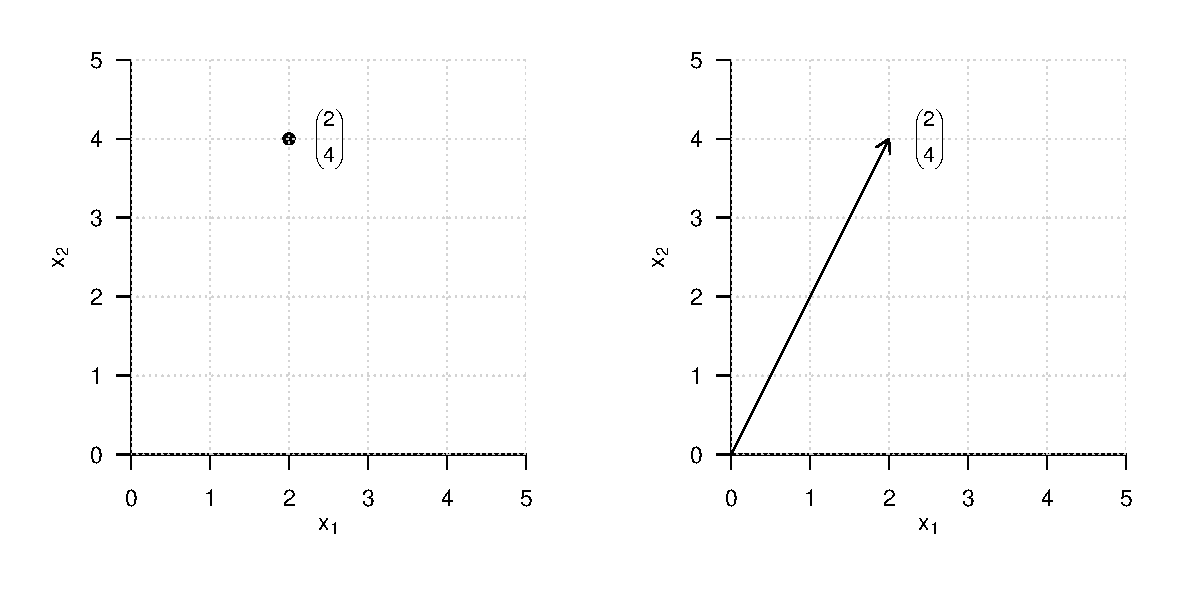
\includegraphics[width=1\linewidth]{2_Abbildungen/mvda_2_vektoren_R2} \end{center}
\end{frame}

\begin{frame}{Reeller Vektorraum}
\protect\hypertarget{reeller-vektorraum-6}{}
\textcolor{darkblue}{Vektoraddition in $\mathbb{R}^2$} \vspace{2mm}
\small \begin{equation}
\begin{pmatrix}
1 \\ 2
\end{pmatrix}
+
\begin{pmatrix}
3 \\ 1
\end{pmatrix}
=
\begin{pmatrix}
4 \\ 3
\end{pmatrix}
\end{equation} \vspace{-2mm}

\begin{center}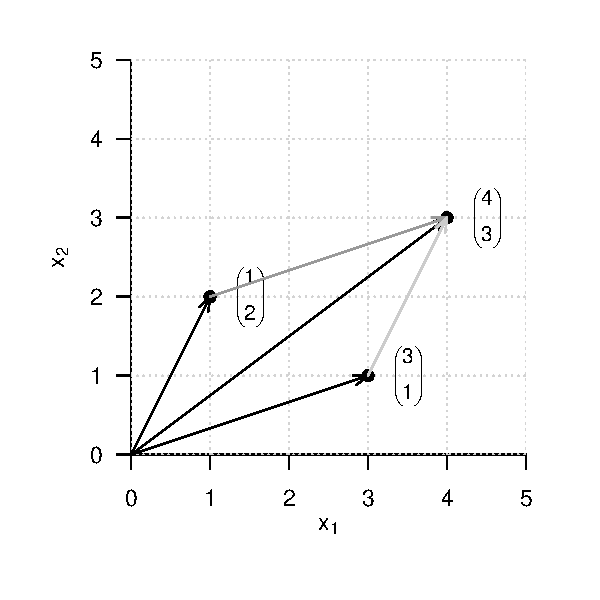
\includegraphics[width=0.5\linewidth]{2_Abbildungen/mvda_2_vektoraddition_R2} \end{center}
\end{frame}

\begin{frame}{Reeller Vektorraum}
\protect\hypertarget{reeller-vektorraum-7}{}
\textcolor{darkblue}{Vektorsubtraktion in $\mathbb{R}^2$} \vspace{2mm}
\small \begin{equation}
\begin{pmatrix}
1 \\ 2
\end{pmatrix}
-
\begin{pmatrix}
3 \\ 1
\end{pmatrix}
=
\begin{pmatrix}
1 \\ 2
\end{pmatrix}
+
\begin{pmatrix}
-3 \\ -1
\end{pmatrix}
=
\begin{pmatrix}
-2 \\ \,\, 1
\end{pmatrix}
\end{equation} \vspace{-2mm}

\begin{center}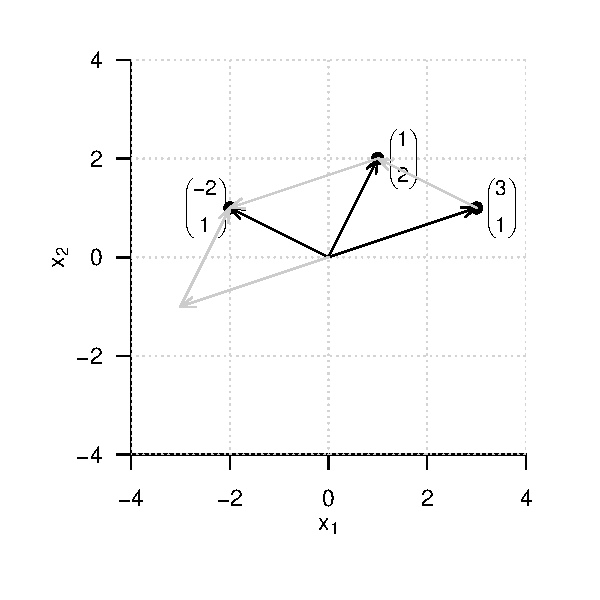
\includegraphics[width=0.5\linewidth]{2_Abbildungen/mvda_2_vektorsubtraktion_R2} \end{center}
\end{frame}

\begin{frame}{Reeller Vektorraum}
\protect\hypertarget{reeller-vektorraum-8}{}
\textcolor{darkblue}{Skalarmultiplikation in $\mathbb{R}^2$}
\vspace{2mm} \small \begin{equation}
3
\begin{pmatrix}
1 \\ 1
\end{pmatrix}
=
\begin{pmatrix}
3 \\ 3
\end{pmatrix}
\end{equation} \vspace{-2mm}

\begin{center}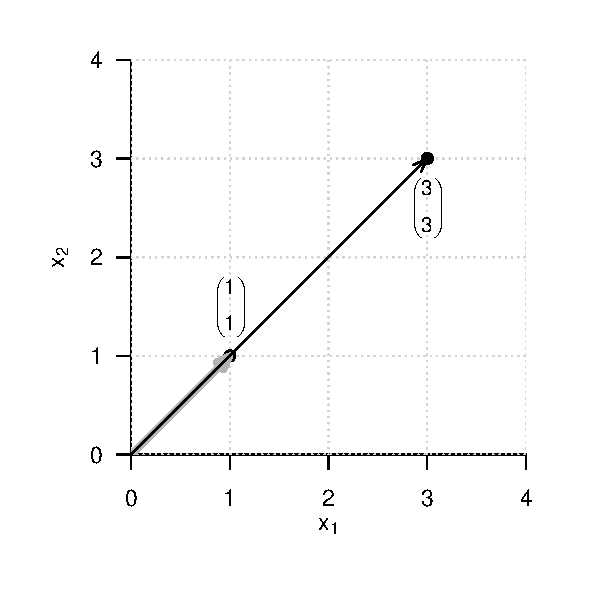
\includegraphics[width=0.5\linewidth]{2_Abbildungen/mvda_2_skalarmultiplikation_R2} \end{center}
\end{frame}

\begin{frame}{}
\protect\hypertarget{section-5}{}
\setstretch{2.5}
\large
\vfill

Reeller Vektorraum

\textbf{Euklidischer Vektorraum}

Lineare Unabhängigkeit

Vektorraumbasen

Selbstkontrollfragen \vfill
\end{frame}

\begin{frame}{Euklidischer Vektorraum}
\protect\hypertarget{euklidischer-vektorraum}{}
\small
\begin{definition}[Skalarprodukt auf $\mathbb{R}^m$]
Das \textit{Skalarprodukt auf $\mathbb{R}^m$} ist definiert als die Abbildung
\begin{equation}
\langle \rangle : \mathbb{R}^m \times \mathbb{R}^m \to \mathbb{R},
(x,y) \mapsto \langle (x,y) \rangle := \langle x,y \rangle := \sum_{i=1}^m x_i y_i.
\end{equation}
\end{definition}

\footnotesize

Bemerkungen

\begin{itemize}
\tightlist
\item
  \justifying Das Skalarprodukt heißt Skalarprodukt, weil es einen
  Skalar ergibt, nicht weil Skalare multipliziert werden.
\item
  Wir sehen später, dass mit der Identifikation
  \(\mathbb{R}^m = \mathbb{R}^{m \times 1}\) und der Matrixtransposition
  gilt, dass \begin{equation}
  \langle x,y \rangle = x^Ty.
  \end{equation}
\end{itemize}
\end{frame}

\begin{frame}[fragile]{Euklidischer Vektorraum}
\protect\hypertarget{euklidischer-vektorraum-1}{}
Beispiel

\footnotesize

Es seien \begin{equation}
x :=
\begin{pmatrix}
1 \\ 2 \\ 3
\end{pmatrix}
\mbox{ und }
y :=
\begin{pmatrix}
2 \\ 0 \\ 1
\end{pmatrix}
\end{equation} Dann ergibt sich \begin{equation}
\langle x,y \rangle
= x_1y_1 + x_2y_2 + x_3y_3
= 1 \cdot 2 + 2 \cdot 0 + 3 \cdot 1
= 2 + 0 + 3
= 5.
\end{equation} \vspace{2mm} \footnotesize

\begin{Shaded}
\begin{Highlighting}[]
\CommentTok{\# Vektordefinitionen}
\NormalTok{x }\OtherTok{=} \FunctionTok{matrix}\NormalTok{(}\FunctionTok{c}\NormalTok{(}\DecValTok{1}\NormalTok{,}\DecValTok{2}\NormalTok{,}\DecValTok{3}\NormalTok{), }\AttributeTok{nrow =} \DecValTok{3}\NormalTok{)}
\NormalTok{y }\OtherTok{=} \FunctionTok{matrix}\NormalTok{(}\FunctionTok{c}\NormalTok{(}\DecValTok{2}\NormalTok{,}\DecValTok{0}\NormalTok{,}\DecValTok{1}\NormalTok{), }\AttributeTok{nrow =} \DecValTok{3}\NormalTok{)}
\end{Highlighting}
\end{Shaded}

\begin{Shaded}
\begin{Highlighting}[]
\CommentTok{\# Skalarprodukt mithilfe von R\textquotesingle{}s komponentenweiser Multiplikation und sum() Funktion}
\FunctionTok{sum}\NormalTok{(x}\SpecialCharTok{*}\NormalTok{y)}
\end{Highlighting}
\end{Shaded}

\begin{verbatim}
> [1] 5
\end{verbatim}

\begin{Shaded}
\begin{Highlighting}[]
\CommentTok{\# Skalarprodukt mithilfe von R\textquotesingle{}s Matrixtransposition und {-}multiplikation}
\FunctionTok{t}\NormalTok{(x) }\SpecialCharTok{\%*\%}\NormalTok{ y}
\end{Highlighting}
\end{Shaded}

\begin{verbatim}
>      [,1]
> [1,]    5
\end{verbatim}
\end{frame}

\begin{frame}{Euklidischer Vektorraum}
\protect\hypertarget{euklidischer-vektorraum-2}{}
\small
\begin{definition}[Euklidischer Vektorraum]
\justifying
Das Tupel $\left((\mathbb{R}^m, +, \cdot), \langle \rangle \right)$ aus dem reellen Vektorraum $(\mathbb{R}^m, +, \cdot)$ und dem Skalarprodukt $\langle \rangle$ auf
$\mathbb{R}^m$ heißt \textit{reeller kanonischer Euklidischer Vektorraum}.
\end{definition}

Bemerkungen

\footnotesize

\begin{itemize}
\tightlist
\item
  \justifying Generell heißt jedes Tupel aus einem Vektorraum und einem
  Skalarprodukt ``Euklidischer Vektorraum''.
\item
  Informell sprechen wir aber oft auch einfach von \(\mathbb{R}^m\) als
  ``Euklidischer Vektorraum'' und insbesondere bei
  \(\left((\mathbb{R}^m, +, \cdot), \langle \rangle \right)\) von
  ``Euklidischen Vektorraum''.
\item
  Ein Euklidischer Vektorraum ist ein Vektorraum mit geometrischer
  Struktur, die durch das Skalarprodukt induziert wird.
\item
  Insbesondere bekommen im Euklidischen Vektorraum Begriffe wie die
  \emph{Länge} eines Vektors, der \emph{Abstand} zweier Vektoren und der
  \emph{Winkel} zwischen zwei Vektoren mithilfe des Skalarproduktes eine
  Bedeutung.
\end{itemize}
\end{frame}

\begin{frame}{Euklidischer Vektorraum}
\protect\hypertarget{euklidischer-vektorraum-3}{}
\setstretch{1.2}
\small
\begin{definition}[Länge, Abstand, Winkel]
$\left((\mathbb{R}^m, +, \cdot), \langle \rangle \right)$ sei der Euklidische Vektorraum.
\begin{itemize}
\item Die \textit{Länge} eines Vektors $x \in \mathbb{R}^m$ ist definiert als
\begin{equation}
\Vert x \Vert := \sqrt{\langle x, x \rangle}.
\end{equation}
\item Der \textit{Abstand} zweier Vektoren $x,y \in \mathbb{R}^m$ ist definiert als
\begin{equation}
d(x,y) := \Vert x - y \Vert.
\end{equation}
\item Der \textit{Winkel} $\alpha$ zwischen zwei Vektoren $x,y \in \mathbb{R}^m$ mit
$x,y \neq 0$ ist definiert durch
\begin{equation}
0 \le \alpha \le \pi \mbox{ und } \cos \alpha
:= \frac{\langle x, y \rangle}{\Vert x \Vert \Vert y \Vert}
\end{equation}
\end{itemize}
\end{definition}

\footnotesize

Bemerkungen

\begin{itemize}
\tightlist
\item
  \(\Vert x \Vert\) heißt auch \emph{Norm von \(x\)} oder
  \emph{\(\ell_2\)-Norm von \(x\)}.
\item
  Ohne Beweis halten wir fest, dass für den Abstand gilt, dass
  \begin{equation}
  d(x,y) \ge 0, d(x,x) = 0, d(x,y) = d(y,x) \mbox{ und } d(x,y) \le d(x,z) + d(z,y).
  \end{equation}
\item
  \(\cos\) ist auf \([0,\pi]\) bijektiv, also invertierbar.
\end{itemize}
\end{frame}

\begin{frame}{Euklidischer Vektorraum}
\protect\hypertarget{euklidischer-vektorraum-4}{}
\textcolor{darkblue}{Vektorlängen in $\mathbb{R}^2$}

\begin{center}\includegraphics[width=0.6\linewidth]{2_Abbildungen/mvda_2_länge_R2} \end{center}
\end{frame}

\begin{frame}[fragile]{Euklidischer Vektorraum}
\protect\hypertarget{euklidischer-vektorraum-5}{}
\textcolor{darkblue}{Vektorlängen in $\mathbb{R}^2$} \footnotesize
\setstretch{1} \begin{equation}
\left\lVert \begin{pmatrix} 2 \\ 0 \end{pmatrix} \right\rVert
= \sqrt{\left\langle \begin{pmatrix} 2 \\ 0 \end{pmatrix}, \begin{pmatrix} 2 \\ 0 \end{pmatrix} \right\rangle}
= \sqrt{2^2 + 0^2}
= \sqrt{4}
= 2.00
\end{equation}

\begin{Shaded}
\begin{Highlighting}[]
\FunctionTok{norm}\NormalTok{(}\FunctionTok{matrix}\NormalTok{(}\FunctionTok{c}\NormalTok{(}\DecValTok{2}\NormalTok{,}\DecValTok{0}\NormalTok{),}\AttributeTok{nrow =} \DecValTok{2}\NormalTok{), }\AttributeTok{type =} \StringTok{"2"}\NormalTok{)             }\CommentTok{\# Vektorlänge = l\_2 Norm}
\end{Highlighting}
\end{Shaded}

\begin{verbatim}
> [1] 2
\end{verbatim}

\begin{equation}
\left\lVert \begin{pmatrix} 2 \\ 2 \end{pmatrix} \right\rVert
= \sqrt{\left\langle \begin{pmatrix} 2 \\ 2 \end{pmatrix}, \begin{pmatrix} 2 \\ 2 \end{pmatrix} \right\rangle}
= \sqrt{2^2 + 2^2}
= \sqrt{8}
\approx 2.83
\end{equation}

\begin{Shaded}
\begin{Highlighting}[]
\FunctionTok{norm}\NormalTok{(}\FunctionTok{matrix}\NormalTok{(}\FunctionTok{c}\NormalTok{(}\DecValTok{2}\NormalTok{,}\DecValTok{2}\NormalTok{),}\AttributeTok{nrow =} \DecValTok{2}\NormalTok{), }\AttributeTok{type =} \StringTok{"2"}\NormalTok{)             }\CommentTok{\# Vektorlänge = l\_2 Norm}
\end{Highlighting}
\end{Shaded}

\begin{verbatim}
> [1] 2.83
\end{verbatim}

\begin{equation}
\left\lVert \begin{pmatrix} 2 \\ 4 \end{pmatrix} \right\rVert
= \sqrt{\left\langle \begin{pmatrix} 2 \\ 4 \end{pmatrix}, \begin{pmatrix} 2 \\ 4 \end{pmatrix} \right\rangle}
= \sqrt{2^2 + 4^2}
= \sqrt{20}
\approx 4.47
\end{equation}

\begin{Shaded}
\begin{Highlighting}[]
\FunctionTok{norm}\NormalTok{(}\FunctionTok{matrix}\NormalTok{(}\FunctionTok{c}\NormalTok{(}\DecValTok{2}\NormalTok{,}\DecValTok{4}\NormalTok{),}\AttributeTok{nrow =} \DecValTok{2}\NormalTok{), }\AttributeTok{type =} \StringTok{"2"}\NormalTok{)             }\CommentTok{\# Vektorlänge = l\_2 Norm}
\end{Highlighting}
\end{Shaded}

\begin{verbatim}
> [1] 4.47
\end{verbatim}
\end{frame}

\begin{frame}{Euklidischer Vektorraum}
\protect\hypertarget{euklidischer-vektorraum-6}{}
\textcolor{darkblue}{Abstände in $\mathbb{R}^2$}

\begin{center}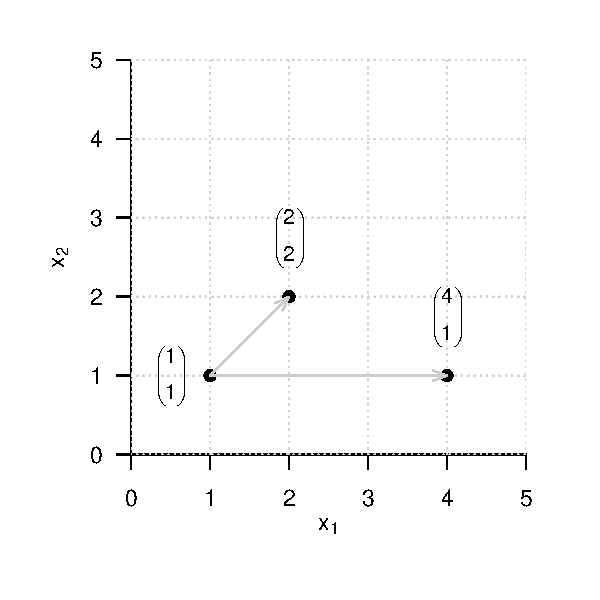
\includegraphics[width=0.6\linewidth]{2_Abbildungen/mvda_2_abstand_R2} \end{center}
\end{frame}

\begin{frame}[fragile]{Euklidischer Vektorraum}
\protect\hypertarget{euklidischer-vektorraum-7}{}
\textcolor{darkblue}{Abstände in $\mathbb{R}^2$} \footnotesize
\vspace{5mm}

\begin{equation}
d\left(\begin{pmatrix} 1 \\ 1 \end{pmatrix}, \begin{pmatrix} 2 \\ 2 \end{pmatrix}\right)
= \left\lVert \begin{pmatrix}  1 \\ 1 \end{pmatrix} - \begin{pmatrix} 2 \\ 2 \end{pmatrix} \right\rVert
= \left\lVert \begin{pmatrix} -1 \\ -1 \end{pmatrix}  \right\rVert
= \sqrt{(-1)^2 + (-1)^2}
= \sqrt{2}
\approx 1.41
\end{equation}

\begin{Shaded}
\begin{Highlighting}[]
\FunctionTok{norm}\NormalTok{(}\FunctionTok{matrix}\NormalTok{(}\FunctionTok{c}\NormalTok{(}\DecValTok{1}\NormalTok{,}\DecValTok{1}\NormalTok{),}\AttributeTok{nrow =} \DecValTok{2}\NormalTok{) }\SpecialCharTok{{-}} \FunctionTok{matrix}\NormalTok{(}\FunctionTok{c}\NormalTok{(}\DecValTok{2}\NormalTok{,}\DecValTok{2}\NormalTok{),}\AttributeTok{nrow =} \DecValTok{2}\NormalTok{), }\AttributeTok{type =} \StringTok{"2"}\NormalTok{)}
\end{Highlighting}
\end{Shaded}

\begin{verbatim}
> [1] 1.41
\end{verbatim}

\vspace{5mm}

\begin{equation}
d\left(\begin{pmatrix} 1 \\ 1 \end{pmatrix}, \begin{pmatrix} 4 \\ 1 \end{pmatrix}\right)
= \left\lVert \begin{pmatrix}  1 \\ 1 \end{pmatrix} - \begin{pmatrix} 4 \\ 1 \end{pmatrix} \right\rVert
= \left\lVert \begin{pmatrix} -3 \\ 0 \end{pmatrix} \right\rVert
= \sqrt{(-3)^2 + 0^2}
= \sqrt{9}
= 3
\end{equation}

\begin{Shaded}
\begin{Highlighting}[]
\FunctionTok{norm}\NormalTok{(}\FunctionTok{matrix}\NormalTok{(}\FunctionTok{c}\NormalTok{(}\DecValTok{1}\NormalTok{,}\DecValTok{1}\NormalTok{),}\AttributeTok{nrow =} \DecValTok{2}\NormalTok{) }\SpecialCharTok{{-}} \FunctionTok{matrix}\NormalTok{(}\FunctionTok{c}\NormalTok{(}\DecValTok{1}\NormalTok{,}\DecValTok{4}\NormalTok{),}\AttributeTok{nrow =} \DecValTok{2}\NormalTok{), }\AttributeTok{type =} \StringTok{"2"}\NormalTok{)}
\end{Highlighting}
\end{Shaded}

\begin{verbatim}
> [1] 3
\end{verbatim}
\end{frame}

\begin{frame}{Euklidischer Vektorraum}
\protect\hypertarget{euklidischer-vektorraum-8}{}
\textcolor{darkblue}{Winkel in $\mathbb{R}^2$}

Kosinus und Arkuskosinus auf \([0,\pi]\)

\begin{center}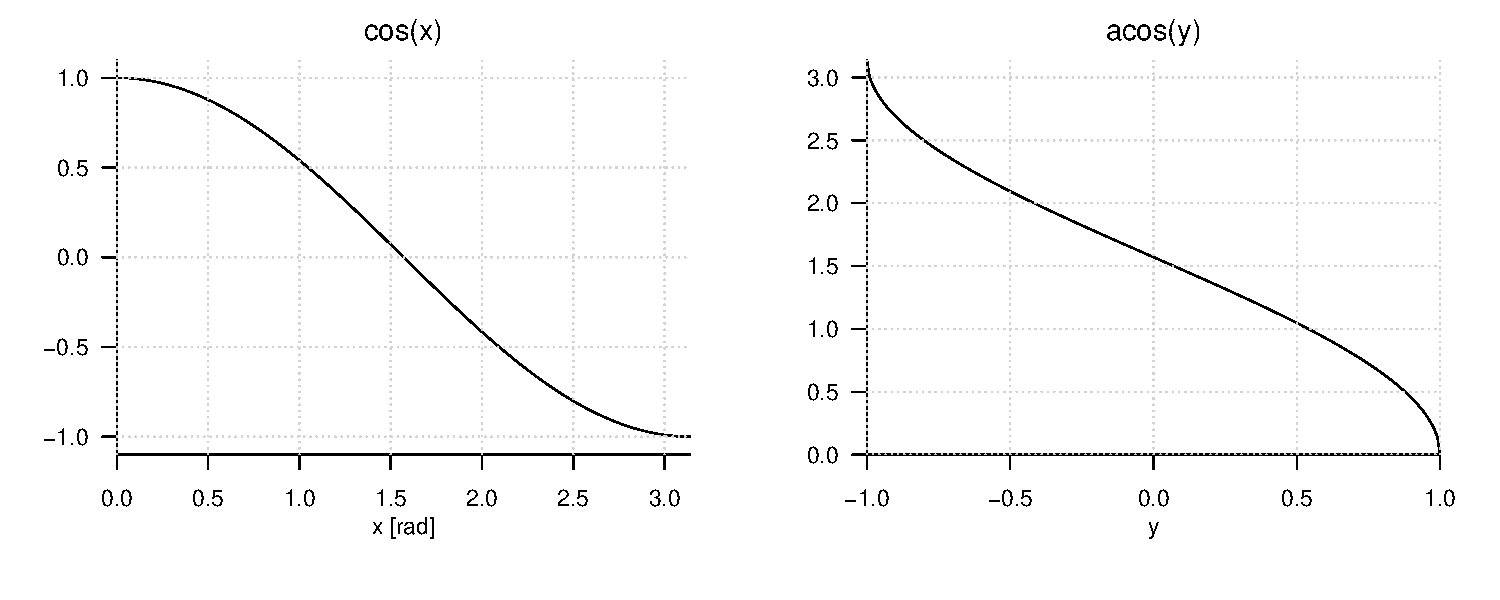
\includegraphics[width=1\linewidth]{2_Abbildungen/mvda_2_kosinus} \end{center}

\vspace{-3mm}
\footnotesize

\begin{equation}
\mbox{deg} = \mbox{rad} \cdot \frac{180}{\pi}, \,
\mbox{rad} = \mbox{deg} \cdot \frac{\pi}{180}
\end{equation} \begin{equation}
0\pi \mbox{ rad }                 = 0.00 \mbox{ rad } = 0  \mbox{ deg }, \,
\frac{\pi}{2} \mbox{ rad } \approx  1.57 \mbox{ rad } = 90 \mbox{ deg }, \,
\pi \mbox{ rad } \approx  3.14 \mbox{ rad } = 180 \mbox{ deg }
\end{equation}
\end{frame}

\begin{frame}{Euklidischer Vektorraum}
\protect\hypertarget{euklidischer-vektorraum-9}{}
\textcolor{darkblue}{Winkel in $\mathbb{R}^2$}

\begin{center}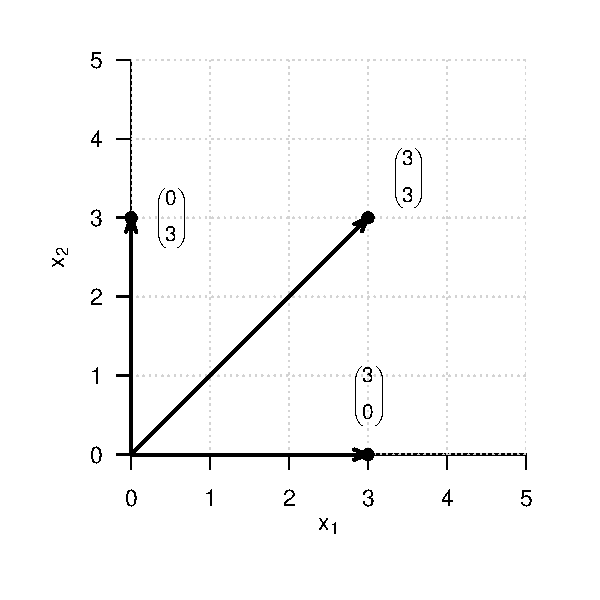
\includegraphics[width=0.6\linewidth]{2_Abbildungen/mvda_2_winkel_R2} \end{center}
\end{frame}

\begin{frame}[fragile]{Euklidischer Vektorraum}
\protect\hypertarget{euklidischer-vektorraum-10}{}
\textcolor{darkblue}{Winkel in $\mathbb{R}^2$}

\footnotesize

Winkel in Radians

\tiny

\begin{equation}
\mbox{acos}
\left(\frac{\left\langle \begin{pmatrix} 3 \\ 0 \end{pmatrix}, \begin{pmatrix} 3 \\ 3 \end{pmatrix} \right\rangle}
           {\left\lVert  \begin{pmatrix} 3 \\ 0 \end{pmatrix} \right\rVert \left\lVert \begin{pmatrix} 3 \\ 3 \end{pmatrix} \right\rVert}
\right)
= \mbox{acos}
\left(\frac{3\cdot 3 + 3 \cdot 0}
           {\sqrt{3^2 + 0^2} \cdot \sqrt{3^2 + 3^2}}
\right)
= \mbox{acos}
\left(\frac{9}
           {3 \cdot \sqrt{18}}
\right)
= \frac{\pi}{4}
\approx 0.785
\end{equation}

\footnotesize

Winkel in Grad

\begin{equation}
0.785 \cdot 180/\pi = 45
\end{equation}

Berechnung in R

\begin{Shaded}
\begin{Highlighting}[]
\NormalTok{x }\OtherTok{=} \FunctionTok{matrix}\NormalTok{(}\FunctionTok{c}\NormalTok{(}\DecValTok{3}\NormalTok{,}\DecValTok{0}\NormalTok{), }\AttributeTok{nrow =} \DecValTok{2}\NormalTok{)                                 }\CommentTok{\# Vektor 1}
\NormalTok{y }\OtherTok{=} \FunctionTok{matrix}\NormalTok{(}\FunctionTok{c}\NormalTok{(}\DecValTok{3}\NormalTok{,}\DecValTok{3}\NormalTok{), }\AttributeTok{nrow =} \DecValTok{2}\NormalTok{)                                 }\CommentTok{\# Vektor 2}
\NormalTok{w }\OtherTok{=} \FunctionTok{acos}\NormalTok{(}\FunctionTok{sum}\NormalTok{(x}\SpecialCharTok{*}\NormalTok{y)}\SpecialCharTok{/}\NormalTok{(}\FunctionTok{sqrt}\NormalTok{(}\FunctionTok{sum}\NormalTok{(x}\SpecialCharTok{*}\NormalTok{x))}\SpecialCharTok{*}\FunctionTok{sqrt}\NormalTok{(}\FunctionTok{sum}\NormalTok{(y}\SpecialCharTok{*}\NormalTok{y)))) }\SpecialCharTok{*} \DecValTok{180}\SpecialCharTok{/}\NormalTok{pi  }\CommentTok{\# Winkel in Grad}
\FunctionTok{print}\NormalTok{(w)}
\end{Highlighting}
\end{Shaded}

\begin{verbatim}
> [1] 45
\end{verbatim}
\end{frame}

\begin{frame}[fragile]{Euklidischer Vektorraum}
\protect\hypertarget{euklidischer-vektorraum-11}{}
\textcolor{darkblue}{Winkel in $\mathbb{R}^2$}

\footnotesize

Winkel in Radians

\tiny

\begin{equation}
\alpha
= \mbox{acos}
\left(\frac{\left\langle \begin{pmatrix} 3 \\ 0 \end{pmatrix}, \begin{pmatrix} 0 \\ 3 \end{pmatrix} \right\rangle}
           {\left\lVert  \begin{pmatrix} 3 \\ 0 \end{pmatrix} \right\rVert \left\lVert \begin{pmatrix} 0 \\ 3 \end{pmatrix} \right\rVert}
\right)
= \mbox{acos}
\left(\frac{3\cdot 0 + 0 \cdot 3}
           {\sqrt{3^2 + 0^2} \cdot \sqrt{0^2 + 3^2}}
\right)
= \mbox{acos}
\left(\frac{0}
           {3 \cdot 3}
\right)
= \frac{\pi}{2}
\approx 1.57
\end{equation}

\footnotesize

Winkel in Grad

\begin{equation}
\frac{\pi}{2} \cdot \frac{180}{\pi} = 90
\end{equation}

Berechnung in R

\begin{Shaded}
\begin{Highlighting}[]
\NormalTok{x }\OtherTok{=} \FunctionTok{matrix}\NormalTok{(}\FunctionTok{c}\NormalTok{(}\DecValTok{3}\NormalTok{,}\DecValTok{0}\NormalTok{), }\AttributeTok{nrow =} \DecValTok{2}\NormalTok{)                                    }\CommentTok{\# Vektor 1}
\NormalTok{y }\OtherTok{=} \FunctionTok{matrix}\NormalTok{(}\FunctionTok{c}\NormalTok{(}\DecValTok{0}\NormalTok{,}\DecValTok{3}\NormalTok{), }\AttributeTok{nrow =} \DecValTok{2}\NormalTok{)                                    }\CommentTok{\# Vektor 2}
\NormalTok{w }\OtherTok{=} \FunctionTok{acos}\NormalTok{(}\FunctionTok{sum}\NormalTok{(x}\SpecialCharTok{*}\NormalTok{y)}\SpecialCharTok{/}\NormalTok{(}\FunctionTok{sqrt}\NormalTok{(}\FunctionTok{sum}\NormalTok{(x}\SpecialCharTok{*}\NormalTok{x))}\SpecialCharTok{*}\FunctionTok{sqrt}\NormalTok{(}\FunctionTok{sum}\NormalTok{(y}\SpecialCharTok{*}\NormalTok{y)))) }\SpecialCharTok{*} \DecValTok{180}\SpecialCharTok{/}\NormalTok{pi     }\CommentTok{\# Winkel in Grad}
\FunctionTok{print}\NormalTok{(w)}
\end{Highlighting}
\end{Shaded}

\begin{verbatim}
> [1] 90
\end{verbatim}
\end{frame}

\begin{frame}{Euklidischer Vektorraum}
\protect\hypertarget{euklidischer-vektorraum-12}{}
\setstretch{1.2}
\small
\begin{definition}[Orthogonalität und Orthonormalität von Vektoren]
\justifying
$\left((\mathbb{R}^m, +, \cdot), \langle \rangle \right)$ sei der Euklidische Vektorraum.
\begin{itemize}
\item Zwei Vektoren $x,y \in \mathbb{R}^m$ heißen \textit{orthogonal}, wenn gilt, dass
\begin{equation}
\langle x, y \rangle = 0
\end{equation}
\item Zwei Vektoren $x,y \in \mathbb{R}^m$ heißen \textit{orthonormal}, wenn gilt, dass
\begin{equation}
\langle x, y \rangle = 0 \mbox{ und } \Vert x \Vert = \Vert y \Vert = 1.
\end{equation}
\end{itemize}
\end{definition}

Bemerkung

\begin{itemize}
\tightlist
\item
  Für orthogonale und orthonormale Vektoren gilt insbesondere auch
  \begin{equation}
  \cos \alpha
  = \frac{\langle x, y \rangle}{\Vert x \Vert \Vert y \Vert}
  = \frac{0}{\Vert x \Vert \Vert y \Vert}
  = 0
  \end{equation} also \begin{equation}
  \alpha = \frac{\pi}{2} = 90^{\circ}
  \end{equation}
\end{itemize}
\end{frame}

\begin{frame}{}
\protect\hypertarget{section-6}{}
\setstretch{2.5}
\large
\vfill

Reeller Vektorraum

Euklidischer Vektorraum

\textbf{Lineare Unabhängigkeit}

Vektorraumbasen

Selbstkontrollfragen \vfill
\end{frame}

\begin{frame}{Lineare Unabhängigkeit}
\protect\hypertarget{lineare-unabhuxe4ngigkeit}{}
\small
\begin{definition}[Linearkombination]
\justifying
$\{v_1, v_2, ..., v_k\}$ sei eine Menge von $k$ Vektoren eines Vektorraums $V$.
Dann ist die \textit{Linearkombination} der Vektoren in $v_1, v_2, ..., v_k$ mit den
skalaren Koeffizienten $a_1, a_2,...,a_k$ definiert als der Vektor
\begin{equation}
w := \sum_{i=1}^k a_i v_i \in V.
\end{equation}
\end{definition}

\footnotesize

Beispiel

Es seien \begin{equation}
v_1 := \begin{pmatrix} 2 \\ 1 \end{pmatrix},
v_2 := \begin{pmatrix} 1 \\ 1 \end{pmatrix},
v_3 := \begin{pmatrix} 0 \\ 1 \end{pmatrix}
\mbox{ und }
a_1 := 2, a_2 := 3, a_3 := 0.
\end{equation} Dann ergibt sich \begin{align}
\begin{split}
w
  = a_1v_1 + a_2v_2 + a_3v_3
& =  2 \cdot \begin{pmatrix} 2 \\ 1 \end{pmatrix}
   + 3 \cdot \begin{pmatrix} 1 \\ 1 \end{pmatrix}
   + 0 \cdot \begin{pmatrix} 0 \\ 1 \end{pmatrix}   \\
& =   \begin{pmatrix} 4 \\ 2 \end{pmatrix}
    + \begin{pmatrix} 3 \\ 3 \end{pmatrix}
    + \begin{pmatrix} 0 \\ 0 \end{pmatrix}          \\
& =   \begin{pmatrix} 7 \\ 5 \end{pmatrix}.
\end{split}
\end{align}
\end{frame}

\begin{frame}{Lineare Unabhängigkeit}
\protect\hypertarget{lineare-unabhuxe4ngigkeit-1}{}
\small
\begin{definition}[Lineare Unabhängigkeit]
\justifying
$V$ sei ein Vektorraum. Eine Menge $W := \{w_1, w_2, ...,w_k\}$ von Vektoren in $V$ heißt
\textit{linear unabhängig}, wenn die einzige Repräsentation des Nullelements
$0 \in V$ durch eine Linearkombination der $w \in W$ die triviale
Repräsentation
\begin{equation}
0 = a_1 w_1 + a_2 w_2 + \cdots + a_k w_k \mbox{ mit } a_1 = a_2 =  \cdots = a_k = 0
\end{equation}
ist. Wenn die Menge $W$ nicht linear unabhängig ist, dann heißt sie \textit{linear abhängig}.
\end{definition}

Bemerkungen

\begin{itemize}
\tightlist
\item
  Prinzipiell müsste man für jede Linearkombination der \(w \in W\)
  prüfen, ob sie Null ist.
\item
  Die beiden folgenden Theoreme zeigen, dass es auch einfacher geht.
\end{itemize}
\end{frame}

\begin{frame}{Lineare Unabhängigkeit}
\protect\hypertarget{lineare-unabhuxe4ngigkeit-2}{}
\small
\begin{theorem}[Lineare Abhängigkeit von zwei Vektoren]
\justifying
\normalfont
$V$ sei ein Vektorraum. Zwei Vektoren $v_1, v_2 \in V$ sind linear abhängig,
wenn einer der Vektoren ein skalares Vielfaches des anderen Vektors ist.
\end{theorem}
\footnotesize

\underline{Beweis} \vspace{1mm}

\(v_1\) sei ein skalares Vielfaches von \(v_2\), also \begin{equation}
v_1 = \lambda v_2 \mbox{ mit } \lambda \neq 0.
\end{equation} Dann gilt \begin{equation}
v_1 - \lambda v_2 = 0.
\end{equation} Dies aber entspricht der Linearkombination
\begin{equation}
a_1v_1 + a_2v_2 = 0
\end{equation} mit \(a_1 = 1 \neq 0\) und \(a_2 = -\lambda \neq 0\). Es
gibt also eine Linearkombination des Nullelementes, die nicht die
triviale Repräsentation ist, und damit sind \(v_1\) und \(v_2\) nicht
linear unabhängig.
\end{frame}

\begin{frame}{Lineare Unabhängigkeit}
\protect\hypertarget{lineare-unabhuxe4ngigkeit-3}{}
\setstretch{1.1}
\small
\begin{theorem}[Lineare Abhängigkeit einer Menge von Vektoren]
\justifying
\normalfont
$V$ sei ein Vektorraum und $w_1,...,w_k \in V$ sei eine Menge von Vektoren in $V$.
Wenn einer der Vektoren $w_i$ mit $i = 1,...,k$ eine Linearkombination der anderen
Vektoren ist, dann ist die Menge der Vektoren linear abhängig.
\end{theorem}

\footnotesize

\underline{Beweis}

Die Vektoren \(w_1,...,w_k\) sind genau dann linear abhängig, wenn gilt,
dass \(\sum_{i=1}^k a_i w_i = 0\) mit mindestens einem \(a_i \neq 0\) .
Es sei also zum Beispiel \(a_j \neq 0\). Dann gilt \begin{equation}
0 = \sum_{i=1}^k a_i w_i = \sum_{i=1, i \neq j}^k a_i w_i + a_jw_j
\end{equation} Also folgt \begin{equation}
a_jw_j  = - \sum_{i=1, i \neq j}^k a_i w_i
\end{equation} und damit \begin{equation}
w_j  = - a_j^{-1}\sum_{i=1, i \neq j}^k a_i w_i = - \sum_{i=1, i \neq j}^k (a_j^{-1}a_i) w_i
\end{equation} Also ist \(w_j\) eine Linearkombination der \(w_i\) für
\(i = 1,...,k\) mit \(i \neq j\). \(\hfill \Box\)
\end{frame}

\begin{frame}{}
\protect\hypertarget{section-7}{}
\setstretch{2.5}
\large
\vfill

Reeller Vektorraum

Euklidischer Vektorraum

Lineare Unabhängigkeit

\textbf{Vektorraumbasen}

Selbstkontrollfragen \vfill
\end{frame}

\begin{frame}{Vektorraumbasen}
\protect\hypertarget{vektorraumbasen}{}
\small
\begin{definition}[Lineare Hülle und Aufspannen]
\justifying
$V$ sei ein Vektorraum und es sei $W := \{w_1,...,w_k\} \subset V$. Dann ist die
\textit{lineare Hülle} von $W$ definiert als die Menge aller Linearkombinationen
der Elemente von $W$,
\begin{equation}
\mbox{Span}(W) := \left\lbrace \sum_{i=1}^k a_iw_i \vert a_1,...,a_k \mbox{ sind skalare Koeffizienten } \right\rbrace
\end{equation}
Man sagt, dass eine Menge von Vektoren $W \subseteq V$ \textit{einen Vektorraum $V$ aufspannt},
wenn jedes $v \in V$ als eine Linearkombination von Vektoren in $W$ geschrieben werden kann.
\end{definition}
\end{frame}

\begin{frame}{Vektorraumbasen}
\protect\hypertarget{vektorraumbasen-1}{}
\small
\begin{definition}[Basis]
$V$ sei ein Vektorraum und es sei $B \subseteq V$. Dann heißt $B$ eine
\textit{Basis von $V$}, wenn
\begin{itemize}
\item die Vektoren in $B$ linear unabhängig sind und
\item die Vektoren in $B$ den Vektorraum $V$ aufspannen.
\end{itemize}
\end{definition}

\begin{theorem}[Eigenschaften von Basen]
\begin{itemize}
\justifying
\normalfont
\item Alle Basen eines Vektorraums beinhalten die gleiche Anzahl von Vektoren.
\item Die Anzahl der Vektoren einer Basis heißt die \textit{Dimension} des Vektorraums.
\item Jede Menge von $m$ linear unabhängigen Vektoren ist Basis eines $m$-dimensionalen Vektorraums.
\end{itemize}
\end{theorem}

Bemerkung

\begin{itemize}
\tightlist
\item
  Wir verzichten auf einen Beweis des sehr tiefen Theorems.
\item
  Vektorräume haben in der Regel unendlich viele Basen.
\end{itemize}
\end{frame}

\begin{frame}{Vektorraumbasen}
\protect\hypertarget{vektorraumbasen-2}{}
\small

\begin{definition}[Basisdarstellung und Koordinaten]
\justifying
$B := \{b_1,...,b_m\}$ sei eine Basis eines $m$-dimensionalen Vektorraumes  $V$
und es sei $v \in V$. Dann heißt die Linearkombination
\begin{equation}
v = \sum_{i = 1}^m c_i b_i
\end{equation}
die \textit{Darstellung von $v$ bezüglich der Basis $B$} und die Koeffizienten
$c_1,...,c_m$ heißen die \textit{Koordinaten von $v$ bezüglich der Basis $B$}.
\end{definition}
\end{frame}

\begin{frame}{Vektorraumbasen}
\protect\hypertarget{vektorraumbasen-3}{}
\small
\begin{theorem}[Eindeutigkeit der Basisdarstellung]
\normalfont
Die Basisdarstellung eines $v \in V$ bezüglich einer Basis $B$ ist eindeutig.
\end{theorem}

\footnotesize

\underline{Beweis} \vspace{1mm}

Ohne Beschränkung der Allgemeinheit nehmen wir an, dass der Vektorraum
von Dimension \(m\) ist. Nehmen wir an, dass zwei Darstellungen von
\(v\) bezüglich der Basis \(B\) existieren, also dass \begin{align}
\begin{split}
v & = a_1 b_1 + \cdots + a_m b_m \\
v & = c_1 b_1 + \cdots + c_m b_m
\end{split}
\end{align} Subtraktion der unteren von dern oberen Gleichung ergibt
\begin{equation}
0 = (a_1 - c_1) b_1 + \cdots + (a_m - c_m) b_m
\end{equation} Weil die \(b_1,...,b_m\) linear unabhängig sind, gilt
aber, dass \((a_i - c_i) = 0\) für alle \(i = 1,...,m\) und somit sind
die beiden Darstellungen von \(v\) bezüglich der Basis \(B\) identisch.

\(\hfill\Box\)
\end{frame}

\begin{frame}{Vektorraumbasen}
\protect\hypertarget{vektorraumbasen-4}{}
\small
\begin{definition}[Orthonormalbasis von $\mathbb{R}^m$]
Eine Menge von $m$ Vektoren $v_1,...,v_m \in \mathbb{R}^m$ heißt
\textit{Orthonormalbasis} von $\mathbb{R}^m$, wenn $v_1,...,v_m$ jeweils die
Länge 1 haben und wechselseitig orthogonal sind, also wenn
\begin{equation}
\langle v_i, v_j \rangle =
\begin{cases}
1   & \mbox{ für } i = j    \\
0   & \mbox{ für } i \neq j
\end{cases}.
\end{equation}
\end{definition}
\end{frame}

\begin{frame}{Vektorraumbasen}
\protect\hypertarget{vektorraumbasen-5}{}
\small

Beispiel 1 \setstretch{1.6}

\footnotesize

Es ist \begin{equation}
B_1 :=
\left\lbrace
\begin{pmatrix}
1 \\ 0
\end{pmatrix},
\begin{pmatrix}
0 \\ 1
\end{pmatrix}
\right\rbrace
\end{equation} eine Orthonormalbasis von \(\mathbb{R}^2\), denn \(B_1\)
besteht aus zwei Vektoren und es gelten \begin{equation}
\left \langle
\begin{pmatrix}
1 \\ 0
\end{pmatrix},
\begin{pmatrix}
1 \\ 0
\end{pmatrix}
\right \rangle
= 1 \cdot 1
+ 0 \cdot 0
= 1 + 0
= 1,
\end{equation} sowie \begin{equation}
\left \langle
\begin{pmatrix}
0 \\ 1
\end{pmatrix},
\begin{pmatrix}
0 \\1
\end{pmatrix}
\right \rangle
= 0 \cdot 0
+ 1 \cdot 1
= 0 + 1
= 1
\end{equation} und \begin{equation}
\left \langle
\begin{pmatrix}
1 \\ 0
\end{pmatrix},
\begin{pmatrix}
0 \\ 1
\end{pmatrix}
\right \rangle
=    1 \cdot 0
  +  0  \cdot 1
= 0 + 0
= 0
\end{equation}
\end{frame}

\begin{frame}{Vektorraumbasen}
\protect\hypertarget{vektorraumbasen-6}{}
\small
\begin{definition}[Kanonische Basis und kanonische Einheitsvektoren]
Die Orthonormalbasis
\begin{equation}
B :=
\left\lbrace
e_1,...,e_m
\vert
e_{i_j} = 1 \mbox{ für } i =  j \mbox{ und } e_{i_j} =  0 \mbox{ für } i \neq j
\right\rbrace
\subset \mathbb{R}^m
\end{equation}
heißt die \textit{kanonische Basis} von $\mathbb{R}^m$ und die $e_{i_j}$ heißen
\textit{kanonische Einheitsvektoren}.
\end{definition}

Beispiele

\begin{itemize}
\item
  \(B_1\) aus Beispiel 1 ist die kanonische Basis von \(\mathbb{R}^2\).
\item
  Die kanonische Basis von \(\mathbb{R}^3\) ist
  \(B := \left\lbrace \begin{pmatrix} 1 \\ 0 \\ 0 \end{pmatrix}, \begin{pmatrix} 0 \\ 1 \\ 0 \end{pmatrix}, \begin{pmatrix} 0 \\ 0 \\ 1 \end{pmatrix} \right\rbrace\).
\end{itemize}
\end{frame}

\begin{frame}{Vektorraumbasen}
\protect\hypertarget{vektorraumbasen-7}{}
\small

Beispiel 2 \setstretch{1.6}

\footnotesize

Es ist auch \begin{equation}
B_2 :=
\left\lbrace
\begin{pmatrix}
\frac{1}{\sqrt{2}} \\ \frac{1}{\sqrt{2}}
\end{pmatrix},
\begin{pmatrix}
- \frac{1}{\sqrt{2}} \\ \quad \frac{1}{\sqrt{2}}
\end{pmatrix}
\right\rbrace
\end{equation} eine Orthonormalbasis von \(\mathbb{R}^2\), denn \(B_2\)
besteht aus zwei Vektoren und es gelten \begin{equation}
\left \langle
\begin{pmatrix}
\frac{1}{\sqrt{2}} \\ \frac{1}{\sqrt{2}}
\end{pmatrix},
\begin{pmatrix}
\frac{1}{\sqrt{2}} \\ \frac{1}{\sqrt{2}}
\end{pmatrix}
\right \rangle
= \frac{1}{\sqrt{2}} \cdot \frac{1}{\sqrt{2}}
+ \frac{1}{\sqrt{2}} \cdot \frac{1}{\sqrt{2}}
= \frac{1}{2} + \frac{1}{2}
= 1,
\end{equation} sowie \begin{equation}
\left \langle
\begin{pmatrix}
- \frac{1}{\sqrt{2}} \\ \quad \frac{1}{\sqrt{2}}
\end{pmatrix},
\begin{pmatrix}
- \frac{1}{\sqrt{2}} \\ \quad \frac{1}{\sqrt{2}}
\end{pmatrix}
\right \rangle
= \left(- \frac{1}{\sqrt{2}} \right)\cdot \left(- \frac{1}{\sqrt{2}} \right)
+ \frac{1}{\sqrt{2}} \cdot \frac{1}{\sqrt{2}}
= \frac{1}{2} + \frac{1}{2}
= 1
\end{equation} und \begin{equation}
\left \langle
\begin{pmatrix}
- \frac{1}{\sqrt{2}} \\ \quad \frac{1}{\sqrt{2}}
\end{pmatrix},
\begin{pmatrix}
  \frac{1}{\sqrt{2}} \\  \frac{1}{\sqrt{2}}
\end{pmatrix}
\right \rangle
= - \frac{1}{\sqrt{2}} \cdot \frac{1}{\sqrt{2}}
  + \frac{1}{\sqrt{2}}   \cdot \frac{1}{\sqrt{2}}
= - \frac{1}{2} + \frac{1}{2}
= 0
\end{equation}
\end{frame}

\begin{frame}{Vektorraumbasen}
\protect\hypertarget{vektorraumbasen-8}{}
Beispiele 1 \& 2

\begin{center}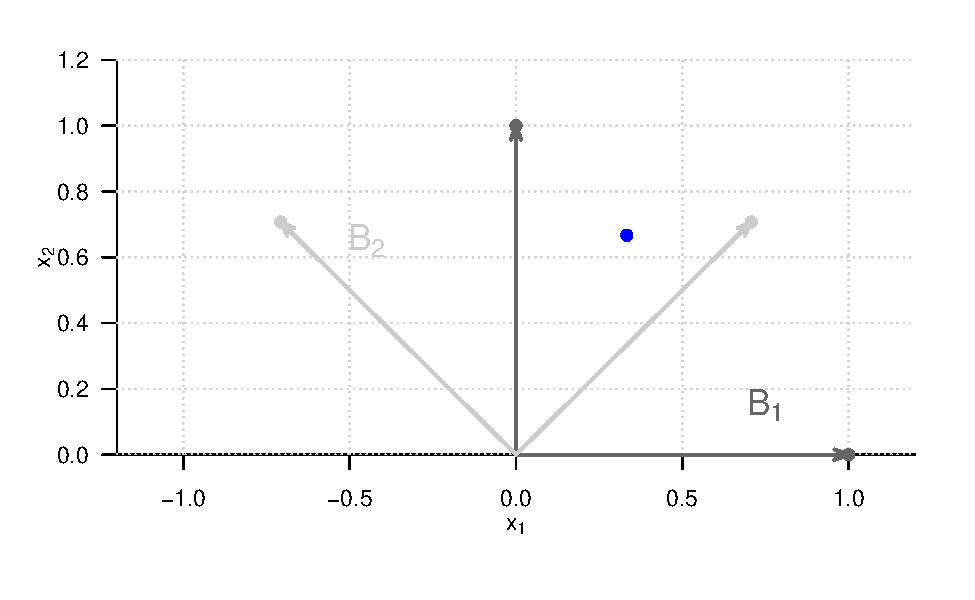
\includegraphics[width=0.8\linewidth]{2_Abbildungen/mvda_2_basen_R2} \end{center}

\small

\begin{itemize}
\tightlist
\item
  \justifying Im Rahmen von Hauptkomponentenranalyse werden wir daran
  interessiert sein, basierend auf den Koordinaten eines Vektors
  bezüglich einer Basis die Koordinaten desselben Vektors bezüglich
  einer anderen Basis zu berechnen.
\end{itemize}
\end{frame}

\begin{frame}{}
\protect\hypertarget{section-8}{}
\setstretch{2.5}
\large
\vfill

Reeller Vektorraum

Euklidischer Vektorraum

Lineare Unabhängigkeit

Vektorraumbasen

\textbf{Selbstkontrollfragen} \vfill
\end{frame}

\begin{frame}{Selbstkontrollfragen}
\protect\hypertarget{selbstkontrollfragen}{}
\footnotesize
\setstretch{1.5}

\begin{enumerate}
\tightlist
\item
  Geben Sie die Definition eines Vektorraums wieder.
\item
  Geben Sie die Definition des reellen Vektorraums wieder.
\item
  Es seien \begin{equation}
  x := \begin{pmatrix} 2 \\ 1 \end{pmatrix}, 
  y := \begin{pmatrix} 0 \\ 1 \end{pmatrix}
  \mbox{ und } 
  a := 2. 
  \end{equation} Berechnen Sie \begin{equation}
  v = a(x+y) \mbox{ und } w = \frac{1}{a}(y-x)
  \end{equation} und überprüfen Sie ihre Rechnung mit R.
\item
  Geben Sie die Definition des Skalarproduktes auf \(\mathbb{R}^m\)
  wieder.
\item
  Für \begin{equation}
  x := \begin{pmatrix} 2 \\ 1 \\ 3 \end{pmatrix},
  y := \begin{pmatrix} 1 \\ 0 \\ 1 \end{pmatrix},
  z := \begin{pmatrix} 3 \\ 1 \\ 0 \end{pmatrix} 
  \end{equation} berechnen Sie \begin{equation}
  \langle x,y \rangle, \langle x, z \rangle, \langle y,z \rangle
  \end{equation} und überprüfen Sie ihre Rechnung mithilfe von R.
\item
  Geben Sie die Definition des Euklidischen Vektorraums wieder.
\item
  Definieren Sie die Länge eines Vektors im Euklidischen Vektorraum.
\item
  Berechnen Sie die Längen der Vektoren \(x,y,z\) aus Aufgabe 5 und
  überprüfen Sie ihre Rechnung mit R.
\end{enumerate}
\end{frame}

\begin{frame}{Selbstkontrollfragen}
\protect\hypertarget{selbstkontrollfragen-1}{}
\footnotesize
\setstretch{1.9}

\begin{enumerate}
\setcounter{enumi}{8}
\tightlist
\item
  Geben Sie Definition des Abstands zweier Vektoren im Euklidischen
  Vektorraum wieder.
\item
  Berechnen Sie \(d(x,y), d(x,z)\) und \(d(y,z)\) für \(x,y,z\) aus
  Aufgabe 5.
\item
  Geben Sie die Definition des Winkels zwischen zwei Vektoren im
  Euklidischen Vektorraum wieder.
\item
  Berechnen Sie die Winkel zwischen den Vektoren \(x\) und \(y\), \(x\)
  und \(z\), sowie \(y\) und \(z\) aus Aufgabe 5 mit R.
\item
  Definieren Sie die Begriffe der Orthogonalität und Orthonormalität von
  Vektoren.
\item
  Definieren Sie den Begriff der Linearkombination von Vektoren.
\item
  Definieren Sie den Begriff der linearen Unabhängigkeit von Vektoren.
\item
  Woran kann man erkennen, dass zwei Vektoren linear abhängig sind?
\item
  Definieren Sie den Begriff der linearen Hülle einer Menge von
  Vektoren.
\item
  Definieren Sie den Begriff der Basis eines Vektorraums.
\item
  Geben Sie das Theorem zu den Eigenschaften von Vektorraumbasen wieder.
\item
  Definieren Sie den Begriff der Basisdarstellung eines Vektors.
\item
  Definieren Sie den Begriff einer Orthonormalbasis von
  \(\mathbb{R}^m\).
\item
  Definieren Sie die kanonische Basis von \(\mathbb{R}^m\)
\end{enumerate}
\end{frame}

\end{document}
